\clearpage
\small
\centering
\textbf{গুরুচণ্ডা৯ প্রকাশিত অন্যান্য কবিতার বই} \\
%\vskip\baselineskip
\raggedright
\scriptsize
চ্যুত; লুনাটিক - দীপাংশু আচার্য \\
বিশ্বাসের কাছে নতজানু - চিরশ্রী দেবনাথ \\
সৌম্য যেভাবে আকাশ দেখেছিল - মণিশঙ্কর বিশ্বাস \\
মন্দ সাইদাতি - জারিফা জাহান \\
পিতৃপরিচয় - বেবী সাউ \\
অযথা চিঠিপত্র বিলি না করে পোস্টাপিসটা খুলে যাচ্ছে সামহন্তা ফুলে – তনুজ \\
সিমোন দ্য নেলসন - রোশনারা মিশ্র ও চিরঞ্জিৎ সামন্ত \\
আগুনপাহাড় - পিনাকী ঠাকুর  \\
এক ব্যাগ ৯০ – ১৯ টি কবিতার বই \\
\hskip \10pt নব্বইয়ের দশকের ১৯ জন কবির ১৯টি বই, একই সঙ্গে। 
\hskip \10pt বিষণ্ণ রূপকথা - অয়ন চক্রবর্তী (দ্বিতীয় মুদ্রণ), সরে দাঁড়ালেন লেন্ডল - অংশুমান কর, জলতলের ফোটোগ্রাফি - আর্যনীল মুখার্জি, যে গান শোনে না কেউ - কল্পর্ষি বন্দোপাধ্যায়, সরু চাকলি - চন্দ্রিল ভট্টাচার্য (দ্বিতীয় সংস্করণ, তৃতীয় মুদ্রণ), কূর্মাবতার - পারমিতা মুন্সি, উজ্জ্বল শ্যামবর্ণা বান্ধবীকে - প্রসূন ভৌমিক, উইকএন্ড - মিতুল দত্ত, সাক্ষরতা মিশন - যশোধরা রায়চৌধুরী, ১৯৮৯ - রোশনারা মিশ্র, উহ্য - শমিত রায়, পড় শুধু স্মৃতি - শান্তনু রায়, যে বয়স হরিণের নয় - শুভেন্দু চট্টোপাধ্যায়, আত্মার আশ্চর্য সেলফি - সার্থক রায়চৌধুরী, যখন ফানুসেরা ওড়ে - সাম্যব্রত জোয়ারদার, পাখিয়াল - সায়ন কর ভৌমিক, ফোনঘর - সুমন মান্না, রেলিং জড়িয়ে প্লাস্টিক - সোমনাথ রায়, লেখো আলো লেখো অন্ধকার - হিন্দোল ভট্টাচার্য \\
ঘেন্না পিত্তি - সোমনাথ রায় \\
অরূপ বৃন্দাবন ও অন্যান্য পদ - সোমনাথ রায় \\
আলির কবিতা - বিশ্বজিৎ চট্টোপাধ্যায় \\
বিনাহ বিতাস - একক \\
\vskip0.5\baselineskip
\raggedleft
\scriptsize
এছাড়া, \\
গুরুচণ্ডা৯র অন্য সব বইয়ের একত্রে সাজানো সমস্ত তথ্য - \\
কোথায় পাওয়া যাবে, দাম কত - সব, \\
নীচের QR কোডটা স্ক্যান করে সাইটে গেলেই পাওয়া যাবে: \\
https://www.guruchandali.com/book.php \\
\vskip0.5\baselineskip
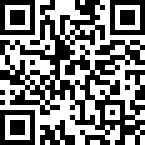
\includegraphics[scale=0.8]{Images/QRCode_2022.png}